\documentclass[12pt,a4paper]{scrartcl}
\usepackage[utf8]{inputenc}
\usepackage{graphicx}
\usepackage{url}
\usepackage{amsmath}
\usepackage{caption}
\usepackage{wrapfig}
\usepackage{eurosym}
\usepackage{biblatex}
\usepackage{url}
\usepackage{color}
\usepackage{listings}
\usepackage{hyperref}
\usepackage[table]{xcolor}
\linespread{1.4}

\definecolor{mygreen}{rgb}{0,0.6,0}
\definecolor{mygray}{rgb}{0.5,0.5,0.5}
\definecolor{mylightgray}{rgb}{0.7,0.7,0.7}
\definecolor{mylightergray}{rgb}{0.9,0.9,0.9}
\definecolor{mymauve}{rgb}{0.58,0,0.82}

\let\origitemize\itemize
\def\itemize{\origitemize\itemsep0pt}

\lstset{ 
  backgroundcolor=\color{white},   
  basicstyle=\ttfamily\footnotesize,          
  breakatwhitespace=false,         
  breaklines=true,  
  commentstyle=\color{mygreen}, 
  escapeinside={\%*}{*)}, 
  extendedchars=true,             
  keepspaces=true,                 
  keywordstyle=\color{blue},
  language=Octave,
  numbers=left,                   
  numbersep=15pt,                  
  numberstyle=\tiny\color{mygray}, 
  showspaces=false,                
  showstringspaces=false,          
  showtabs=false,                  
  stringstyle=\color{mymauve},
  tabsize=2,
  title=\lstname,
  captionpos=b
}

\renewcommand*\lstlistingname{Codebeispiel}    %Rename Listings

\renewcommand*\thesection{\arabic{section}}

\makeatletter
\renewcommand\subparagraph{\@startsection{subparagraph}{5}{\parindent}%
    {3.25ex \@plus1ex \@minus .2ex}%
    {0.75ex plus 0.1ex}% space after heading
    {\normalfont\normalsize\bfseries}}
\makeatother

\begin{document}
\title{
\begin{figure}[!h]
	\centering
    
\includegraphics[width=8cm]{title.pdf}
\end{figure}
}
\subtitle{User Manual and Documentation}
\author{Maria Floru\ss}
\maketitle
\newpage

\section*{User Manual}
\subsection*{Controls}

\subsubsection*{General}
\begin{tabular}{l | p{3cm} | p{6cm} }
 & Keyboard & GamePad\\ \hline
restart level & R & Back\\
\end{tabular}
\\
\subsubsection*{Circle}
\begin{tabular}{l | p{3cm} | p{6cm} }
 & Keyboard & GamePad\\ \hline
move left & A & Left Thumbstick - left\\
move right & D & Left Thumbstick - right\\
press button & S & Left Trigger\\
\end{tabular}
\\
\subsubsection*{Square}
\begin{tabular}{l | p{3cm} | p{6cm} }
 & Keyboard & GamePad\\ \hline
move left & Left Arrow & Right Thumbstick - left\\
move right & Right Arrow & Right Thumbstick - right\\
jump & Up Arrow & Right Bumper\\
press button & Down Arrow & Right Trigger
\end{tabular}
\\
\subsubsection*{Menu}
\begin{tabular}{l | p{3cm} | p{6cm} }
 & Keyboard & GamePad\\ \hline
toggle menu & Escape & Start\\
navigate menu & Arrow Keys & DPad\\
confirm & Enter & A
\end{tabular}
\\
\subsubsection*{Debug}
\begin{tabular}{l | p{3cm}}
 & Keyboard \\ \hline
toggle physics drawing & F9 \\
cycle through debug info & F10 \\
cycle through visual helpers & F11\\
zoom in & Numpad + \\
zoom out & Numpad -
\end{tabular}


\section*{Game Mechanics}
You start in the game with two players. They have to help each other to get to the end of the level (usually on the right). As you enter the tunnel at the end of the level you will be redirected to the next level.

There are several game objects, that can help the players to reach their goal.

\subsection*{Buttons}
Buttons can be triggered by either square or circle exclusively. There are two kinds of buttons:
\begin{description}
\item[blue buttons] can toggle the state of a platform or obstacle. If you press it once, the platform will stay visible. 
\item [yellow buttons] need to be pressed down in order to move or toggle platforms and obstacles.
\end{description}

\subsection*{Platforms}
Platforms are horizontal, physical objects, that help the players getting somewhere. They can be triggered by a button. As there are two buttons, there are two kinds of platforms. 
\begin{description}
\item[blue platforms] will be toggled on and off by a blue button. Once the button is pressed the platform stays visible until the button is pressed again.  
\item [yellow platforms] will be triggered by a yellow button. They are only active as long as the button is pressed. They can either move or be toggled on and off.
\end{description}

\subsection*{Obstacles}
Obstacles are vertical, physical objects, that usually are in the players way. They can be triggered by a button. As there are two buttons, there are two kinds of platforms. 
\begin{description}
\item[blue obstacles] will be toggled on and off by a blue button. Once the button is pressed the platform stays visible until the button is pressed again.  
\item [yellow obstacles] will be triggered by a yellow button. They are only active as long as the button is pressed. They can only be toggled on and off.
\end{description}

\newpage

\section*{Idea and Design}

\subsection*{Finding an Idea}
At the beginning I played 'Brothers - A Tale of Two Sons', developed by Starbreeze Studios and published by 505 Games released on 7 August 2013. In this game the player takes control over two brothers, who are controlled by the left and right part of the gamepad respectively. This singleplayer co-op principle was very impressive to me and I started thinking about games like this, where one player controls two characters. When we started with the lecture I already had some ideas about how my game could have looked like. There were many ideas, of which many did not make it into the final game due to complexity and time constraints.
 
Ever since I started developing the game I wanted to make it aesthetically appealing as well, even though the art would not influence my grading.

\subsection*{Development}
\subsubsection*{Box2D}
As the physics are a major part of this game and I didn't have the time to do it all by myself, I used Box2D as a physics engine. At the beginning this was a bit cumbersome, because I didn't know how to use it properly, but in the end I figured it out and everything went better than expected. 

\subsubsection*{Level Generation}
In order to get the collision of my relatively complex levels I wrote a level generator, which would allow me to draw my levels as .bmp files. A red dot would mark the beginning of a static physical body, which would contain one or more edges. A black dot would determine the end of an edge and the beginning of a new one. The gray lines would connect the red and black dots. 

\begin{figure}[!h]
    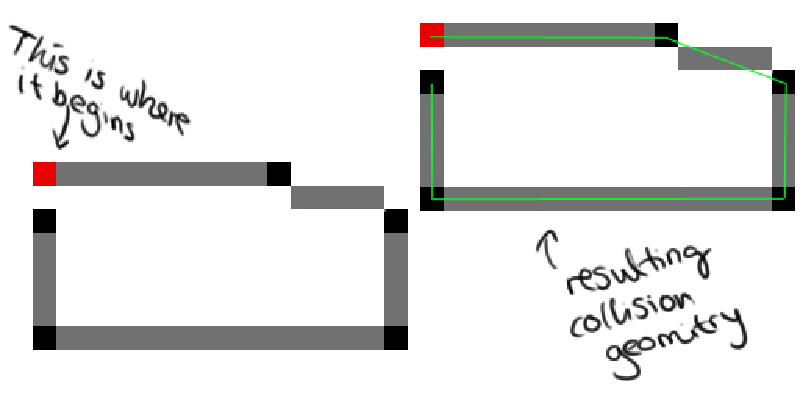
\includegraphics[width=\textwidth]{collision.pdf}
\end{figure}

\subsubsection*{Configuration Files}
To describe my levels, e.g. the position of the game objects, the maximum speed of the players or the connection of a button to the according platform, I used a configuration file reader, written by Manuel Maier. This allowed me to balance my game and create new levels very easily. Internally the game objects and players use the configuration files to initialize themselves. 
\\\\
Excerpt of a configuration file:
\begin{lstlisting}
[circleTrigger]
type = toggleButton
drawOrder = 20
position = 1145, 457
proximityRadius = 20
master = circle
state = inactive
onButtonOn = togglePlattform
onButtonOff = togglePlattform
textureOn = objects/button_circle_1_on
textureOff = objects/button_circle_1_off
\end{lstlisting}

\subsubsection*{Camera}
The camera is a modified version of Khalid Abuhakmeh's post on stackoverflow.com: \url{http://stackoverflow.com/a/723918} (date: 2014-09-09). 

I had to add some features, because I had two players, which should be followed by the camera. In order to achieve this, I used a proxy game object, which is positioned in between circle and square. I also added view bounds, to make sure the view port won't leave the level.  

\subsubsection*{Audio}
For audio I'm using XACT which comes with XNA. It is mainly used to play the background music in a level. Due to the complexity of the API I wrote an \lstinline{AudioManager} that wraps the API and provides just the functionality that is needed for my game.

The following files are taken from bigcat\_smauls at
 \url{http://www.freesound.org/people/bigcat_smauls/}

\begin{itemize}
\item 222802\_\_bigcat-smauls\_\_like-a-dream-loop.wav
\item 223722\_\_bigcat-smauls\_\_keep-at-it-loop.wav
\item 222800\_\_bigcat-smauls\_\_gur-durge-loop.wav
\end{itemize}

Licensed under the Creative Commons 0 License, these items are in the public domain.

\subsection*{Future Concepts}

The following is a collection of concepts that sadly did not make it into the final game due to complexity and time constraints.  

\begin{figure}[!h]
    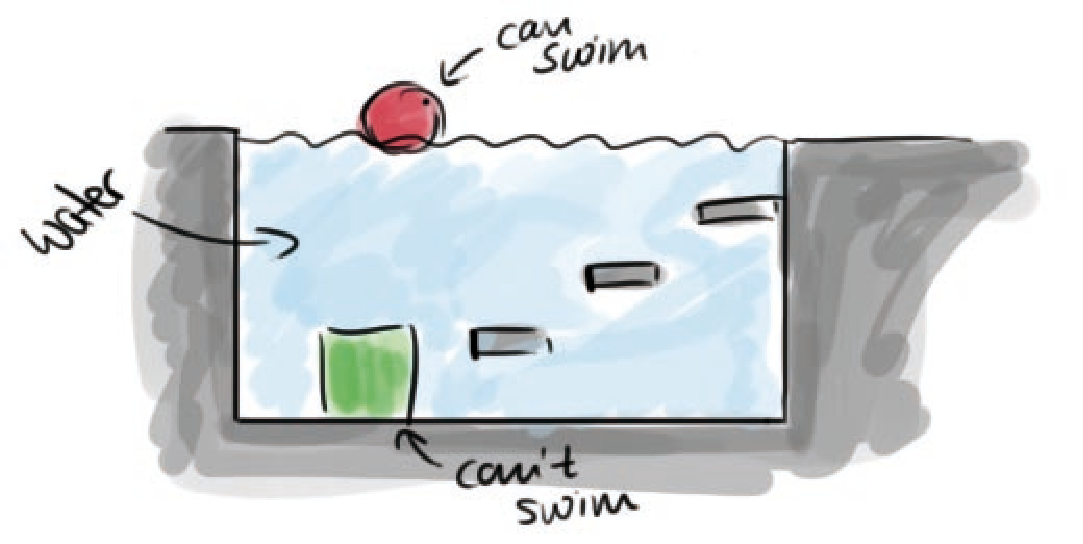
\includegraphics[width=\textwidth]{water.pdf}
\end{figure}

\begin{figure}[!h]
    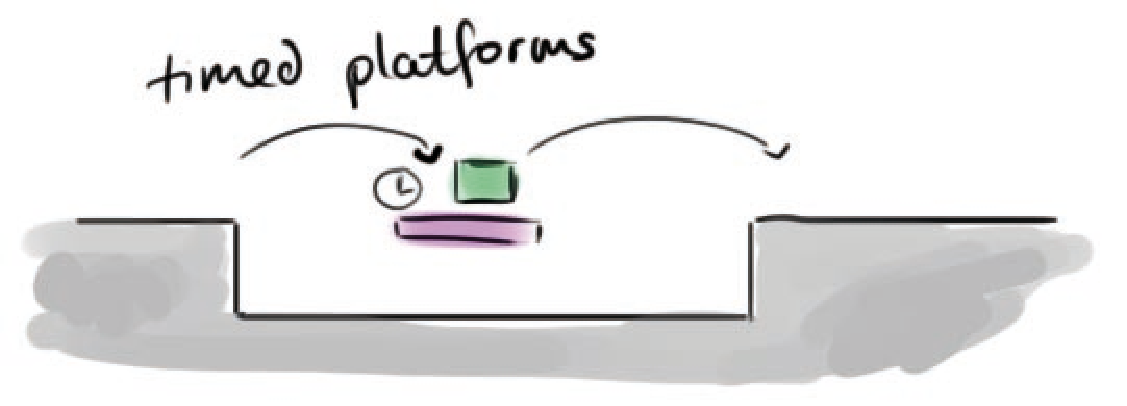
\includegraphics[width=\textwidth]{timed.pdf}
\end{figure}

\begin{figure}[!h]
    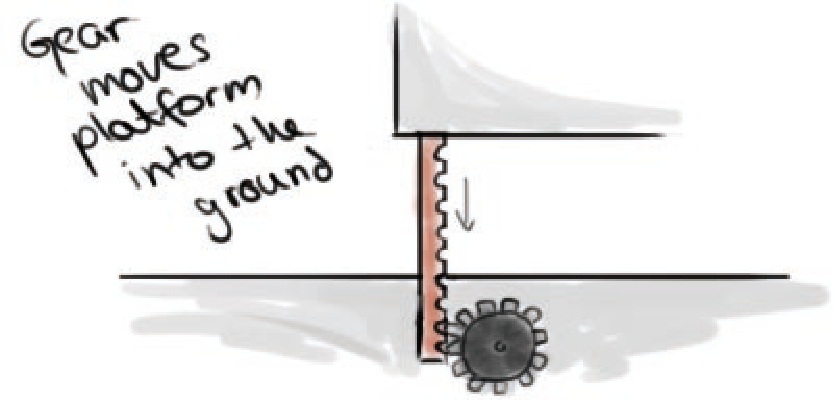
\includegraphics[width=\textwidth]{gear.pdf}
\end{figure}

\begin{figure}[!h]
    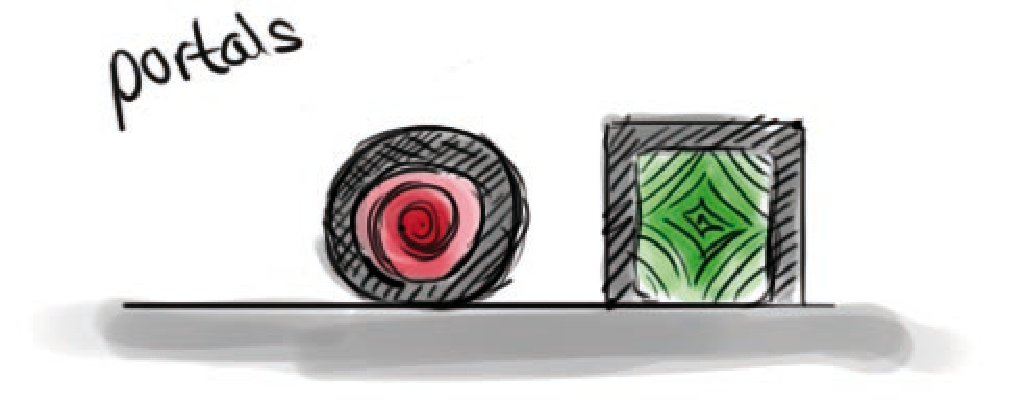
\includegraphics[width=\textwidth]{portals.pdf}
\end{figure}

\begin{figure}[!h]
    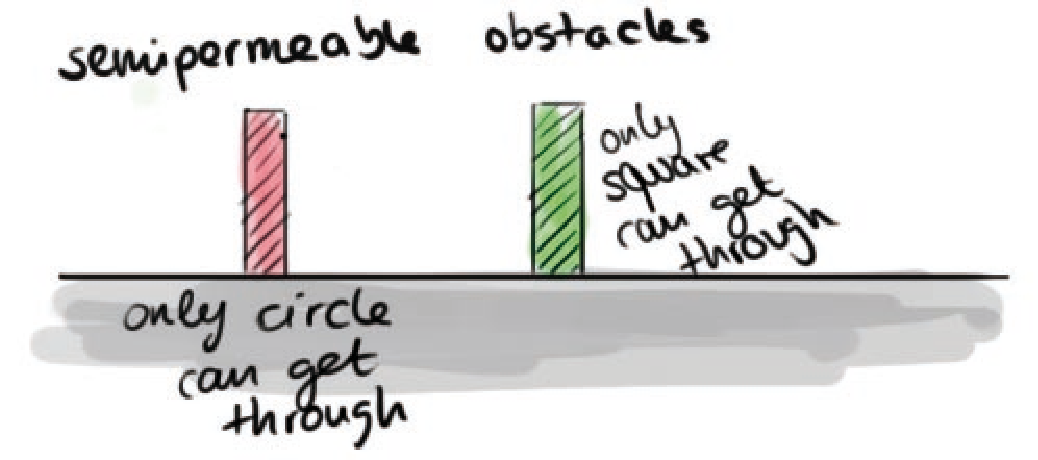
\includegraphics[width=\textwidth]{semi.pdf}
\end{figure}

\begin{figure}[!h]
    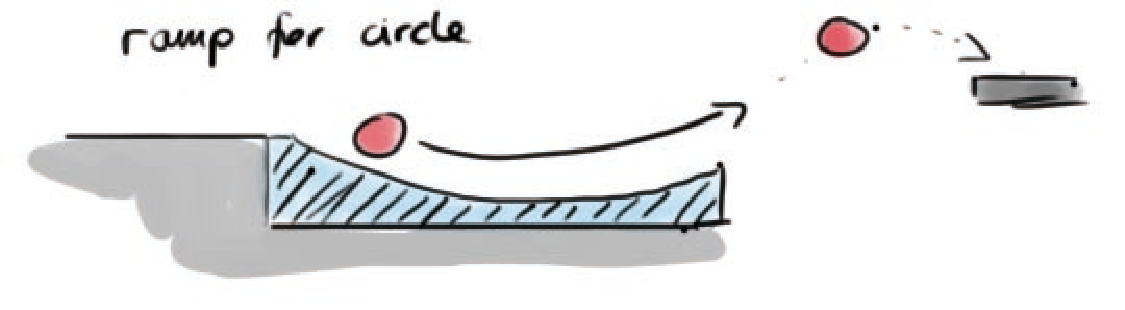
\includegraphics[width=\textwidth]{ramp.pdf}
\end{figure}




\end{document}